%============================================================================
% tento soubor pouzijte jako zaklad
% (c) 2008 Michal Bidlo
% E-mail: bidlom AT fit vutbr cz
%============================================================================
% kodovaní: utf-8 (zmena prikazem iconv, recode nebo cstocs)
%----------------------------------------------------------------------------
% zpracování: make, make pdf, make desky, make clean
% připomínky posílejte na e-mail: bidlom AT fit.vutbr.cz
% vim: set syntax=tex encoding=utf-8:
%============================================================================
\documentclass[english,cover]{fitthesis} % odevzdani do wisu - odkazy, na ktere se da klikat
%\documentclass[cover,print]{fitthesis} % pro tisk - na odkazy se neda klikat
%\documentclass[english,print]{fitthesis} % pro tisk - na odkazy se neda klikat
%      \documentclass[english]{fitthesis}
% * Je-li prace psana v anglickem jazyce, je zapotrebi u tridy pouzit 
%   parametr english nasledovne:
%      \documentclass[english]{fitthesis}
% * Neprejete-li si vysazet na prvni strane dokumentu desky, zruste 
%   parametr cover

% zde zvolime kodovani, ve kterem je napsan text prace
% "latin2" pro iso8859-2 nebo "cp1250" pro windows-1250, "utf8" pro "utf-8"
%\usepackage{ucs}
\usepackage[utf8]{inputenc}
\usepackage[T1, IL2]{fontenc}
\usepackage{url}
\DeclareUrlCommand\url{\def\UrlLeft{<}\def\UrlRight{>} \urlstyle{tt}}

%zde muzeme vlozit vlastni balicky
\usepackage{amsmath}
\usepackage{amsthm}
\usepackage{color}
\usepackage{comment}
\usepackage{graphicx}
\usepackage{caption}
\usepackage{subcaption}
\newtheorem{math_def}{Definition}[chapter] % 3. parametr zajisti cislovani "<sekce>.<číslo definice>"
\newcommand{\term}[1]{\emph{#1}}           % novy termin v textu prace
\newcommand{\todo}[1]{{\color{red} #1}}
\newcommand{\uncertain}[1]{{\color{magenta} #1}}
\newcommand{\note}[1]{{\color{green} #1}}
\newcommand{\vars}[1]{{\mathbf{#1}}} % matematicke vyrazy - mnozina
\newcommand{\ignore}[1]{} % komentar v radku


% =======================================================================
% balíček "hyperref" vytváří klikací odkazy v pdf, pokud tedy použijeme pdflatex
% problém je, že balíček hyperref musí být uveden jako poslední, takže nemůže
% být v šabloně
\ifWis
\ifx\pdfoutput\undefined % nejedeme pod pdflatexem
\else
  \usepackage{color}
  \usepackage[unicode,colorlinks,hyperindex,plainpages=false,pdftex]{hyperref}
  \definecolor{links}{rgb}{0.4,0.5,0}
  \definecolor{anchors}{rgb}{1,0,0}
  \def\AnchorColor{anchors}
  \def\LinkColor{links}
  \def\pdfBorderAttrs{/Border [0 0 0] }  % bez okrajů kolem odkazů
  \pdfcompresslevel=9
\fi
\fi

%Informace o praci/projektu
%---------------------------------------------------------------------------
\projectinfo{
  %Prace
  project=DP,            %typ prace BP/SP/DP/DR
  year=2012,             %rok
  date=\today,          %datum odevzdani
  %Nazev prace
  title.cs={Aplikace Bayesovských sítí},  %nazev prace v cestine
  title.en={Bayesian Networks Applications}, %nazev prace v anglictine
  %Autor
  author={David Chaloupka},   %jmeno prijmeni autora
  author.title.p=Bc., %titul pred jmenem (nepovinne)
  %author.title.a=PhD, %titul za jmenem (nepovinne)
  %Ustav
  department=UITS, % doplnte prislusnou zkratku: UPSY/UIFS/UITS/UPGM
  %Skolitel
  supervisor=František V. Zbořil, %jmeno prijmeni skolitele
  supervisor.title.p=doc.~Ing.,   %titul pred jmenem (nepovinne)
  supervisor.title.a={CSc.},    %titul za jmenem (nepovinne)
  %Klicova slova, abstrakty, prohlaseni a podekovani je mozne definovat 
  %bud pomoci nasledujicich parametru nebo pomoci vyhrazenych maker (viz dale)
  %===========================================================================
  %Klicova slova
  keywords.cs={Klíčová slova v českém jazyce.}, %klicova slova v ceskem jazyce
  keywords.en={Klíčová slova v anglickém jazyce.}, %klicova slova v anglickem jazyce
  %Abstract
  abstract.cs={Výtah (abstrakt) práce v českém jazyce.}, % abstrakt v ceskem jazyce
  abstract.en={Výtah (abstrakt) práce v anglickém jazyce.}, % abstrakt v anglickem jazyce
  %Prohlaseni
  declaration={Prohlašuji, že jsem tuto bakalářskou práci vypracoval samostatně pod vedením pana ...},
  %Podekovani (nepovinne)
  acknowledgment={Zde je možné uvést poděkování vedoucímu práce a těm, kteří poskytli odbornou pomoc.} % nepovinne
}

%Abstrakt (cesky, anglicky)
%\abstract[cs]{Do tohoto odstavce bude zapsán výtah (abstrakt) práce v českém jazyce.}
%\abstract[en]{Do tohoto odstavce bude zapsán výtah (abstrakt) práce v anglickém jazyce.}

%Klicova slova (cesky, anglicky)
%\keywords[cs]{Sem budou zapsána jednotlivá klíčová slova v českém jazyce, oddělená čárkami.}
%\keywords[en]{Sem budou zapsána jednotlivá klíčová slova v anglickém jazyce, oddělená čárkami.}

%Prohlaseni
%\declaration{Prohlašuji, že jsem tuto bakalářskou práci vypracoval samostatně pod vedením pana X...
%Další informace mi poskytli...
%Uvedl jsem všechny literární prameny a publikace, ze kterých jsem čerpal.}

%Podekovani (nepovinne)
%\acknowledgment{V této sekci je možno uvést poděkování vedoucímu práce a těm, kteří poskytli odbornou pomoc
%(externí zadavatel, konzultant, apod.).}

\begin{document}
  % Vysazeni titulnich stran
  % ----------------------------------------------
  \maketitle
  % Obsah
  % ----------------------------------------------
  \tableofcontents
  
  % Seznam obrazku a tabulek (pokud prace obsahuje velke mnozstvi obrazku, tak se to hodi)
  % \listoffigures
  % \listoftables 

  % Text prace
  % ----------------------------------------------

  








%end-of-inserted-header
%=========================================================================
% (c) Michal Bidlo, Bohuslav Křena, 2008

\chapter{Introduction}

Bayesian networks represent a subclass of probabilistic graphical models and they serve as a tool for modeling probability distributions of random variables. Bayesian networks were originally used to evaluate medical data of a patient in order to determine probability of him having a certain disease\,--\,a situation with many unknown facts (eg. missing medical history or unknown results of possible tests). Since then there have been many other applications such as inspection of pedigree trees in genetics or general classification tasks.

The main advantage of Bayesian networks lies in their inherent property that, thanks to conditional dependency and independency between variables, they represent the probability distribution in a very compact way in terms of space complexity. Construction of Bayesian networks for some concrete problem is a complicated process involving complex algorithms, enough input data and, in most cases, expert knowledge. Another problem is answering queries over the underlaying probability distribution of a Bayesian network, so called inference.

The aim of this thesis is to present techniques of learning Bayesian networks, both in terms of conditional probability tables as well as in terms of structure and show possible application domains. Inference is narrowed down to stochastic approaches because other ways, are very complex. Still all forms of inference will be mentioned at least on the level of basic concept, since it is a fundamental part of theory of Bayesian networks.

\todo{popis jednotlivých kapitol}































\chapter{Theory of Bayesian networks}
This chapter will present theoretical foundations for understanding Bayesian networks and performing computation over them. Studying Bayesian networks (further abbreviated as BNs) is challenging both because of necessary mathematical rigor as well as for the need of efficient non-trivial algorithms to construct them and then to provide answers for probability queries.

First will be established notation used in this thesis and necessary overview of probability theory. Then we will proceed to the theory of Bayesian networks, explain their advantages and proceed to construction and inference techniques.


\section{Preliminaries}
At first we need to establish notation and explain basic facts regarding mathematical probability because, as will be shown later, Bayesian networks are graphical models for joint probability distributions.

\subsection{Philosophical views}
Probability is usually interpreted as degree of belief in occurrence of a particular event, eg. probability of a fair die rolling a six is $1/6$. Although probability is expressed as a~real number between zero and one, the ground truth is that in the end one and only one \emph{concrete} event is observed. In the case of a die, one concrete number is rolled regardless what the probabilities were. Although our intuition and general experience proves it to be true in our macroscopic world, objects in the microscopic world of quantum mechanics actually are probabilistic in nature and, a particle for example, is in many quantum states at the same time. The particle is then described by so called wave function $\Psi$; then $\vert\Psi\vert^2$ describes density probability as a function of space and time coordinates. Despite the obvious differences, certain qualities of both these worlds can be described by the same mathematical apparatus which is probability theory. \todo{cite physics from grammar school?}

Somewhat close to probability theory is the theory of fuzzy sets which operates with membership functions. These functions describe degrees of truth, eg. that a person is regarded as young or old. The main difference, when compared to probability, is that in fuzzy sets theory an object may have more than one quality to some degree and there is no ground truth or observation that would strictly place a person to one single category.


\subsection{Probability distributions}
Lets begin by defining what a probability distribution is when there is only one single random variable.
\begin{math_def}\label{def_prob_distribution}
    $P(X)$ is discrete probability distribution of discrete random variable $X$ such that:
    \begin{itemize}
        \item $X$ can be assigned any value from the set $\lbrace x_1, x_2, \dots \rbrace$ which is finite or denumerable.
        \item $\forall i: P(X = x_i) \geq 0$
        \item $\Bigl( \sum_i P(X = x_i) \Bigr) = 1$
    \end{itemize}
\end{math_def}

Notice that random variables are denoted by capital letters $X, Y, E$ etc., concrete values of random variables (instantiations) are denoted by small letters such as $x$. Further we'll use bold capital letters to denote sets of random variables such as $\vars{X}$ and their instantiation with bold small letters such as $\vars{x}$.

Probability distributions of more than one random variable are called \term{joint probability distributions}. For example if we were to study a simultaneous throw with two dices, black and white, we would get joint probability distribution $P(X_{black},X_{white})$. In this probability distribution we know how likely is every single outcome of a throw. In this case there are $6 \times 6 = 36$ possibilities so the $P(X_{black},X_{white})$ function would have 36 entries if represented by a table.

So far we've described probability distributions of variables that don't depend on any other variables. \term{Conditional probability distribution} of variables $\vars{X}$ depending on variables $\vars{E}$ is denoted $P(\vars{X}\mid\vars{E})$. Such expression is often read as "probability of $\vars{X}$ given $\vars{E}$" where $\vars{E}$ are called \term{evidence} or \term{observed} variables. Conditional probability distribution can be seen as a collection of probability distributions of variables $\vars{X}$ for every possible assignment to variables $\vars{E}$.

Probability distributions introduced so far describe so called \term{prior probabilities} which are applicable in situations when no observation has been made and hence everything is governed purely by probability. If, on the other hand, we know concrete value of some random variable then we speak of \term{posterior probability} and the observed variables are called \term{evidence variables}. Posterior and prior probability distributions are not the same in general because observation of a variable may affect distribution of other variables. This topic will be studied further in context of Bayesian networks and conditional dependencies they encode.


\subsection{Factors}
When reasoning about Bayesian networks we express probability distributions as so called \term{factors}. Factors are interesting for us because factor operations correspond to mathematical operations we need to do with probability distributions in order to answer queries in a~Bayesian network. 
\begin{math_def}\label{def_factor}
    Factor $\phi$ is a function $\phi: X_1 \times X_2 \times \dotsm \times X_k \rightarrow \mathbb{R}_0^+$. The non-empy set $\lbrace X_1, X_2, \dots, X_k \rbrace$ is called scope of the factor $\phi$.
\end{math_def}
According to the definition of a factor and to the definition \ref{def_prob_distribution} of a discrete probability distribution, probability distributions are special cases of factors. They both require their values to be non-negative and, in addition, every probability distribution must sum to one. A~factor, of course, may sum to one too in which case we say it is \term{normalized}.

There are 4 operations over factors we will need further in this thesis\,--\,pointwise product, marginalization, conditioning and renormalization. Definitions below are inspired by description of these operations in~\cite{russell_norvig_ed2, pgm}

\subsubsection{Pointwise product}
Pointwise product of factors $\phi_1$ and $\phi_2$ is a factor $\psi$, denoted $\psi = \phi_1 \cdot \phi_2$, defined as follows. The scope of $\psi$ is $scope(\phi_1) \cup scope(\phi_2)$. Let $scope(\phi_1) = \lbrace X_1, \dots, X_m, Y_1, \dots, Y_n \rbrace$ and $scope(\phi_2) = \lbrace Y_1, \dots, Y_n, Z_1, \dots, Z_k \rbrace$ where $\lbrace X_1, \dots, X_m \rbrace$ and $\lbrace Z_1, \dots, Z_k \rbrace$ are disjoint. For every assignment $x_1, \dots, x_m, y_1, \dots, y_n, z_1, \dots, z_k$ of variables in $scope(\psi)$ the value of $\psi$ is given as:
$$\psi(x_1, \dots, x_m, y_1, \dots, y_n, z_1, \dots, z_k)
= \phi_1(x_1, \dots, x_m, y_1, \dots, y_n) \cdot \phi_2(y_1, \dots, y_n, z_1, \dots, z_k)
$$

Please note that it is also possible for the sets $\lbrace X_i \rbrace, \lbrace Y_i \rbrace,\lbrace Z_i \rbrace$ to be empty (of course, according to the definition~\ref{def_factor}, factor must have at least one variable in it's scope).

Factor representation of a joint probability distribution $P(X,\dots,Z)$ is straightforward\,--\,simply put $\phi(x,\dots,z) = P(x,\dots,z)$ for every assignment $x,\dots,z$ of variables $X,\dots,Z$. In this case probabilities of all possible assignments must necessarily sum to one since $P(X,\dots,Z)$ is a~probability distribution. For further reference, this summation is denoted $\sum_{X,\dots,Z} P(x,\dots,z) = 1$.

Lets examine the case of a conditional probability distribution $P(\vars{X}\mid\vars{E})$. Suppose that, according to the established notation, $\vars{X}$ and $\vars{E}$ are sets of variables rather than single variables. Then $scope(\phi)$ is $\vars{X} \cup \vars{E}$ but probability of all possible assignments to $\vars{X}$ and $\vars{E}$ doesn't sum to one! This is because the conditional probability distribution $P(\vars{X}\mid\vars{E})$ is more like a collection of probability distributions of variables $\vars{X}$ for every assignment to $\vars{E}$. So, for any concrete assignment $\vars{e}$ of evidence variables $\vars{E}$, the probability distribution $P(\vars{X}\mid\vars{e})$ again sums to one, ie. $\sum_\vars{X} P(\vars{x}\mid\vars{e}) = 1$.

\subsubsection{Marginalization}
Marginalization of a factor $\phi$ over variables $\vars{Y}$ is operation of summing out these variables, effectively producing factor $\psi$. Then $scope(\psi) = scope(\phi) \setminus \vars{Y}$ and for every assignment $\vars{x}$ of variables in $scope(\phi)$ holds that $\psi(\vars{x}) = \sum_\vars{Y} \phi(\vars{x},\vars{y})$.

\subsubsection{Conditioning}
Conditioning is operation used when there is some observed evidence $\vars{e}$ of variables $\vars{E}$. By conditioning we set probabilities of all events inconsistent with observed evidence to 0. Of~course the resulting factor won't be normalized in general.

\subsubsection{Renormalization}
Renormalization of factor $\phi$ ensures that all values of the factor sum to one. Suppose that $\vars{X} = scope(\phi)$ and let $\alpha = \sum_\vars{X} \phi(\vars{x})$ be normalizing constant. Values of the resulting factor $\psi$ are given for every assignment $\vars{x}$ of variables $\vars{X}$ as $\psi(\vars{x}) = \phi(\vars{x}) / \alpha$.

It may be useful to point out that renormalization makes sense only for factors that don't represent conditional probability distributions.




\section{Bayesian networks}
Question might be why to use Bayesian networks? First of all, having a complicated joint probability distribution with many random variables inevitably leads to a potentially enormously large table that would represent such probability distribution. Lets assume we have binary random variables $X_1, X_2, \dots$ Then for representing distribution $P(X_1)$ we would need a table with two entries, for distribution $P(X_1, X_2)$ the table would have four entries and a general distribution $P(X_1, \dots, X_k)$ would have a table with $2^k$ entries. This exponential growth brings several problems:
\begin{itemize}
    \item Table completely describing a joint probability distribution may be too big to store. That is because the table would hold probability of every possible event separately in it's own record.
    \item Even if the table could be stored, performing calculations over it (e.g. factor marginalization or factor multiplication) would not be efficient. In fact operations such as exact inference are known to be NP-hard in the number of variables~\cite{pgm}.
    \item In order to construct probability table for a joint probability distribution:
    \begin{enumerate}
        \item[a)] We would require huge amount of training data to create an accurate statistical model from, since we would essentially count occurrences of every single event (ie. of possible assignments to all random variables) and finally divide these counts by the total number of all training examples.
        \item[b)] We would need a human expert to determine the probability of every possible assignment to random variables. This is generally not possible because all probabilities would be near to zero and human experts are simply not able to correctly capture probabilities on this level~\cite{pgm}.
    \end{enumerate}
\end{itemize}

As will be shown later, Bayesian networks couple with the problem of exponential growth of records in probability tables by having several smaller conditional probability distributions (factors) based on dependencies between random variables. Product of all these conditional probabilities (factors) gives the underlaying joint probability distribution which would, if represented directly, require an exponentially bigger table.

\begin{math_def}\label{def_bayesian_network}
    Bayesian network $G$ is a directed acyclic graph where each node represents a~random variable and oriented edges between nodes express direct dependencies between random variables.
\end{math_def}

The definition of Bayesian network (further abbreviated BN) implies several things. Acyclic and directed properties tell us that there is a hierarchy of nodes in terms of parent-child relation, meaning that child random variable $C$ is dependent on its parent random variables $P_1, \dots, P_m$ (also denoted $Parents(C)$). This conditional probability distribution $P(C \mid Parents(C))$ is usually\footnote{For purposes of this thesis, we assume probability distributions of discrete, not continuous, variables whose events are from a finite set. Such probability distribution can be expressed by a table.} expressed via a \term{Conditional Probability Table (CPT)} that defines probability distribution of variable $C$ for every possible assignment of variables $Parents(C)$. Of course, for every assignment $p_1,\dots,p_m$ of variables $Parents(C)$ must hold that $\sum_C P(c \mid p_1, \dots, p_m) = 1$. Otherwise $P(C \mid Parents(C))$ would not be a probability distribution (by definition~\ref{def_prob_distribution}).

We say that Bayesian network $G$ with nodes $\lbrace X_1, \dots, X_k\rbrace$ induces joint probability distribution $P(X_1, \dots, X_k)$ as follows:
\begin{equation}\label{eq:bn_joint}
    P(X_1, \dots, X_k) = \prod_{i=1}^k P(X_i \mid Parents(X_i))
\end{equation}
Equivalent statement is that $P(X_1, \dots, X_k)$ factorizes over BN $G$ if the equation \eqref{eq:bn_joint} holds. This is because the terms $P(X_i \mid Parents(X_i))$ are \term{factors} and by constructing a~Bayesian network we can factorize otherwise very space-consuming CPD of $P(X_1, \dots, X_k)$ into several smaller CPDs $P(X_i \mid Parents(X_i))$, one for every node $X_i$.

I've devised a proof that $P(X_1, \dots, X_k)$ induced by a BN $G$ is indeed a probability distribution, when assuming that every factor $P(X_i \mid Parents(X_i))$ in $G$ also is a probability distribution. Main purpose of this proof is to provide the reader with some familiarity when mathematically reasoning about BNs because similar tricks will be used later on. Core of the proof is to show that both axioms of a probability distribution (Definition \ref{def_prob_distribution}) are satisfied\footnote{Because of long expressions in the following two paragraphs, $Pars(X)$ denotes $Parents(X)$.}:
\begin{enumerate}
   \item $P(X_1, \dots, X_k) \geq 0$:
       Trivial since factors $P(X_i \mid Parents(X_i))$ are assumed to be valid probability distributions. Then, by definition of probability distribution~\ref{def_prob_distribution}, we know that $\forall i: P(X_i \mid Parents(X_i)) \geq 0$. And product of non-negative numbers (factors) is also non-negative.
   \item $\sum P(x_1, \dots, x_k) = 1$:
       If the remaining variables $X_1, \dots, X_k$ are all independent, then by definition of independent random variables $P(X_1, \dots, X_k) = P(X_1) \dotsm P(X_k)$. So the sum can be written as $\sum P(x_1, \dots, x_k) = \sum_{X_1} P(x_1) \sum_{X_2} P(x_2) \dotsm \sum_{X_k} P(x_k)$. By assumption, all factors are valid probability distributions, so $\sum_{X_k} P(x_k) = 1$. Then $\sum_{X_1} P(x_1) \sum_{X_2} P(x_2) \dotsm \sum_{X_k} P(x_k) = \sum_{X_1} P(x_1) \sum_{X_2} P(x_2) \dotsm 1$. Thus we have eliminated variable $X_k$ and transformed the problem to $\sum P(x_1, \dots, x_{k-1}) = 1$. By eliminating all remaining variables the same way, we get $\sum P(x_1, \dots, x_k) = 1$.
       
       If there is a direct dependency between some two variables, lets relabel the variables so that their indices correspond to a topological sort of the given BN (every BN is a~DAG, so a topological sort exists).  Then we can rewrite the inspected summation in the form $\sum P(x_1, \dots, x_k) = \sum_{X_1} P(x_1 | Pars(X_1)) \sum_{X_2} P(x_2 | Pars(X_2)) \dotsm \sum_{X_k} P(x_k | Pars(X_k))$ because, thanks to the topological sort, all parent variables of a variable $X_i$ must have smaller index that $i$. Also note that the maximal element $X_k$ has no child. By assumption, $P(X_k \mid Pars(X_k))$ is a probability distribution, so $\sum_{X_k} P(x_k \mid Pars(X_k)) = 1$. By substituting the term $\sum_{X_k} P(x_k \mid Pars(X_k))$ in the summation we eliminate the variable $X_k$ and transform the problem to question if $\sum P(x_1, \dots, x_{k-1}) = 1$ which we approach analogically.
\end{enumerate}


\subsection{Flow of probabilistic influence}
To describe how observing certain facts propagates through a Bayesian network and how it affects probability distributions of unobserved variables on qualitative level, lets introduce \term{flow of probabilistic influence}. Flow of influence also enables us to formally capture conditional dependency and/or independency of random variables in a BN given some facts.
\begin{math_def}
    Let $G$ be a Bayesian network with nodes $X_1, X_2, \dots, X_k$ and let $\vars{Z}$ be a~set of observed variables. Connected undirected trail $X_a - X_{a+1} - \dots - X_b$ given facts $\vars{Z}$ is active iff
    \begin{itemize}
        \item For every so called "V-structure" $X_{i-1} \rightarrow X_i \leftarrow X_{i+1}$ on the trail is $X_i \in \vars{Z}$.
        \item No other node of given trail is in $\vars{Z}$.
    \end{itemize}
    Notes: V-structure is defined as a segment of trail in form $X_{i-1} \rightarrow X_i \leftarrow X_{i+1}$ (in this case, edge directions do matter). Also note that the trail may contain duplicate nodes.
\end{math_def}

\begin{math_def}
    Let $G$ be a Bayesian network, $X,Y$ two of it's nodes and $\vars{Z}$ observed variables. We say that $X,Y$ given $\vars{Z}$ are d-separated in $G$ iff there is no active trail between $X$ and $Y$ given $\vars{Z}$.
    
    Note: $X$ and $Y$ being d-separated given $\vars{Z}$ is equivalent to $X$ and $Y$ being conditionally independent given $\vars{Z}$, denoted $X \perp Y \mid \vars{Z}$.
\end{math_def}

Using d-separation (direction-dependent separation) we can quite elegantly determine if observation of a variable $X$ can or cannot affect distribution of some other random variable. Clearly two random variables that are directly connected are dependent. But we can also examine other than these intuitively obvious relations. Also please note that whether two random variables $X,Y$ are independent in Bayesian network depends on our observations $\vars{Z}$ as it can activate some trails in V-structures just as it can deactivate direct segments of other trails.

To understand better the notion of active trails and d-separation see examples in Figure~\ref{fig:bn_d-separation}. In Figure~\ref{fig:bn_d-separation_a} you can see that if we have information about the accident variable, then knowing whether there is a traffic jam doesn't affect probability of hearing sirens and vice versa because knowing the accident variable deactivates all trails between T and H.
In Figure~\ref{fig:bn_d-separation_b} we can see an activated V-structure R$\rightarrow$T$\leftarrow$A. When we know whether there is a traffic jam then, intuitively, an accident decreases probability of being it in a rush hour because an accident can cause a traffic jam by itself. Similarly if it is not a rush hour then probability of there being an accident goes up. This is an example of inter-causal reasoning.

\begin{figure}[h]
\begin{center}
    \begin{subfigure}[b]{0.4\linewidth}
        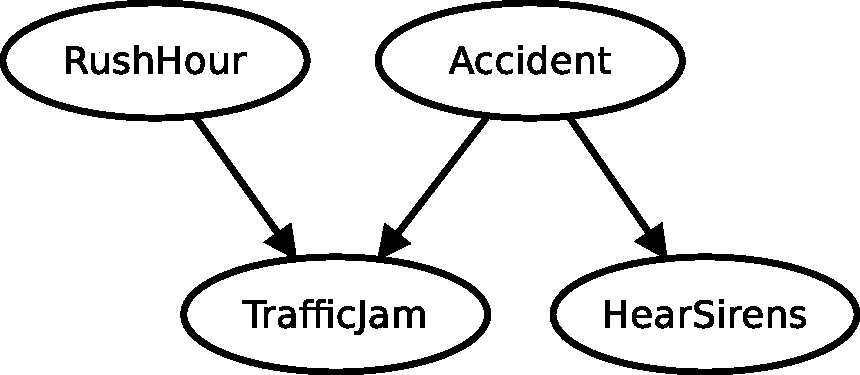
\includegraphics[scale=0.45]{fig/bn-d_sep}
        \caption{$T \perp H \mid A$}
        \label{fig:bn_d-separation_a}
    \end{subfigure}
    \quad
    \begin{subfigure}[b]{0.4\linewidth}
        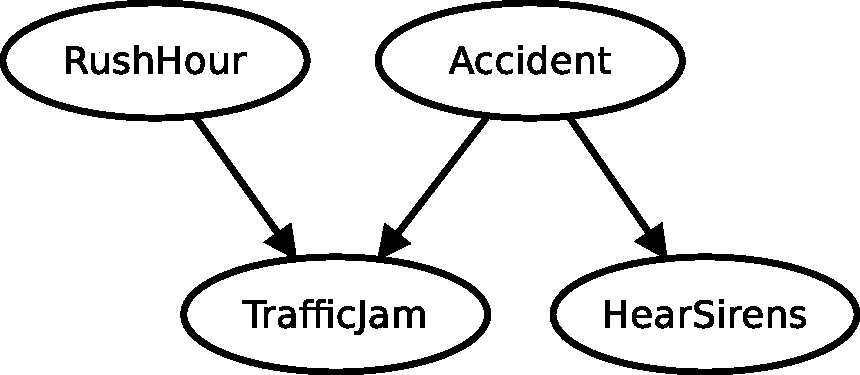
\includegraphics[scale=0.45]{fig/bn-d_sep}
        \caption{$R\not\perp A \mid T$ (active trail R-T-A-H)}
        \label{fig:bn_d-separation_b}
    \end{subfigure}
    \caption{Examples of d-separation and flow of influence.}
    \label{fig:bn_d-separation}
\end{center}
\end{figure}

It might be useful to explicitly point out what the notation $P(X_i \mid Parents(X_i))$ tells us in context of d-separation. It is a fact frequently used in mathematical derivations in context of BNs that, when given all parents $Parents(X_i)$ of a variable $X_i$, the variable is independent on all indirect parents of $X_i$ in the network.













\section{Inference in Bayesian networks}
There are several types of queries that might be asked in context of a Bayesian network. Most often by inference in BNs is meant computing the posterior probability distribution for a set of query variables $\vars{X}$ given values of evidence variables $\vars{E}$. Mathematically the task is to compute the probability distribution $P(\vars{X} \mid \vars{E})$. Another type of query is so called \term{maximum a~posteriori} (abbreviated as MAP) that is finding $arg\ max_\vars{X} P(\vars{X} \mid \vars{E})$. MAP is basically used for finding out the most probable cause (concrete assignment of variables $\vars{X}$) for observations $\vars{E}$. Practical example could be getting the most probable word (sequence of letters) that corresponds to classifier output for a segmented picture containing that word. Although this is an example more frequently used in context of Markov networks.

Inference in a BN may be carried out in many ways depending on nature of the query and precision requirements. Exact inference is relatively straightforward in terms of mathematical description and naive algorithmic implementation but exhibits serious running-time disadvantage\,--\,exponential running time in the number of variables in the worst case. On the other hand, approximate inference methods allow us to answer queries more quickly but precision of the solution may be questionable, especially for very rare events.

\todo{include types of queries\,--\,diagnostic, causal, intercausal, mixed? (Russell, Norvig 2ed page 448 (466 pdf))}

\subsection{Sum-product}
Probably the simplest method for computing a conditional probability query is called sum-product. The problem at hand is to compute conditional probability distribution $P(\vars{X} \mid \vars{e})$ where $\vars{X}$ is one or more variables, $\vars{e}$ is an assignment to evidence variables $\vars{E}$ and $\vars{Y}$ variables that are neither query nor evidence variables. The query is computed according to Bayes' theorem as follows:
\begin{equation*}
P(\vars{X} \mid \vars{e})
 = \frac{P(\vars{X}, \vars{e})} {P(\vars{e})}
 = \frac{\sum_\vars{Y} P(\vars{X}, \vars{y}, \vars{e})}{\sum_{\vars{X},\vars{Y}} P(\vars{x}, \vars{y}, \vars{e})}
\end{equation*}
The denominator is constant and since $P(\vars{X} \mid \vars{e})$ has to be a probability distribution, we can simply omit the denominator and in the end normalize numerator by some constant $\alpha$. Hence we can write
\begin{equation*}
P(\vars{X} \mid \vars{e})
 = \alpha \sum_\vars{Y} P(\vars{X}, \vars{y}, \vars{e})
\end{equation*}
Computation of this expression using the sum-product method means performing four steps:
\begin{enumerate}
	\item reducing all factors in the Bayesian network by evidence $\vars{e}$,
	\item multiplying reduced factors all together producing single joint factor $P(\vars{X},\vars{Y},\vars{e})$ which is not a probability distribution because, in general, all values of the factor don't sum to one,
	\item marginalizing over the variables $\vars{Y}$ (non-query and non-evidence variables) and finally
	\item renormalizing the resulting factor, obtaining the joint probability distribution $P(\vars{X},\vars{e})$.
\end{enumerate}

Every item of the sum in numerator, ie. probability of every possible assignment to variables $\vars{Y}$, can be written according to the joint probability distribution represented by a BN (definition~\eqref{eq:bn_joint}) as a~product of conditional probabilities of all variables in given BN. This explains the name of this inference method\,--\,we effectively compute many products of conditional probabilities and sum over variables $\vars{Y}$.

Sum-product inference algorithm has, from its nature, exponential running time in the number of variables because it effectively generates the whole joint probability distribution encoded by given Bayesian network and size of a table representing any joint probability distribution has been earlier shown to be exponential in the number of variables. Because of this quality, the sum-product method is suitable only for inference in considerably small networks.

\begin{comment}
\uncertain{
Formally, exact number of operations carried out in the nominator sum during the sum-product inference can be determined as follows. Let $m$ be the number of all variables, let $n$~be the number of non-query and non-evidence variables $\vars{Y}$ and let $k$~be the number of possible assignments to a variable. The numerator summation unrolls to $k^n$ items, each item being a product of all $m$ factors which means $k^n (m-1)$ multiplications and $k^n - 1$ additions. Therefore the overall running time is roughly $O(m k^n)$.}
\end{comment}


\subsection{Variable elimination}
Variable elimination algorithm can be seen as a somewhat smarter implementation of the sum-product algorithm explained above. Again, we answer the given query by multiplying all factors of the BN and summing out $\vars{Y}$ variables. The innovative ideas behind variable elimination are:
\begin{itemize}
	\item Suppose we sum over many variables in a product of factors, say one of these variables is $V$. Then factors whose scopes don't contain $V$ are irrelevant for the summation over~$V$ and hence these factors can be factored out in front of the summation over~$V$. This way we can push all summations as far to the right as possible, so that each summation is done only over product of factors containing the variable $V$ being summed out. What is the benefit for us? It can be shown~\cite{pgm} that running time of variable elimination depends on the size of the largest immediate factor during the summing-out process. When we sum only over product of factors containing variable $V$, the resulting immediate factor is the smallest possible. Because problem of determining the optimal order of elimination is NP-hard, greedy heuristics are usually used instead~\cite{pgm}.
	\item By definition of a conditional probability distribution, it holds for any instantiation of parent variables that $\sum_V P(v \mid Parents(V)) = 1$. So, when computing aposterior probability distribution $P(\vars{X} \mid \vars{e})$, any node (factor) $V$ that is not an ancestor of a~query or evidence variable can be ommited because, thanks to the order of elimination of variables, the term $\sum_V P(v \mid Parents(V))$ will be the rightmost summation (the innermost). So summing out $V$ is equivalent to totally excluding variable $V$ from the BN. Implementation can be recursively done in the way of eliminating all leaf nodes that are not in $\vars{X} \cup \vars{E}$ and performing the same operation for as long as some node gets removed~\cite[p.~510]{russell_norvig_ed2}.
\end{itemize}

\todo{řeči kolem, algoritmus, časová složitost, kliky}

Running time of variable elimination in polytrees is $O(n)$~\cite[p.~510]{russell_norvig_ed2}, therefore it is a good method for answering individual queries $P(X \mid \vars{e})$ where $X$ is single variable. Analogically we can effectively compute probability distribution for small number of query variables $\vars{X}$ by computing individual distributions $P(X_i \mid \vars{e})$ and returning $P(\vars{X}) = \prod_i P(X_i \mid \vars{e})$.

Running time in multiply connected networks is exponential in general but it can be coped with by clustering algorithms that transform multiply connected network into a~polytree.

\subsection{Belief propagation}
Belief propagation~\cite{pgm} is an approximate inference algorithm from the family of so called \term{message passing algorithms}. The main idea is that nodes in the BN exchange information about their believes (probability distributions affected by evidence) and the whole network converges to some solution close to true posterior probability. As methods from this family are far from trivial and they are not the aim of this thesis, we won't pay deeper attention to them.
\begin{comment}
\note{Cluster graphs and \term{running intersection property}: Nodes $C_i \subseteq \lbrace X_1, \dots, X_n \rbrace$ and sepsets $S_{i,j} \subseteq C_i \cup C_j$ such that for each factor $\phi$ exists $C_i$: $scope(\phi) \subseteq C_i$.
For each variable $X$ the nodes $C_i$ and sepsets containing $X$ form a tree (ie. no cycle and single unbroken component)\,--\,cycle would mean that a node would get information about variable $X$ twice and the probabilities would go up and up. If some node with $X$ would be isolated from others, it would not get the belief updates. Bethe cluster automatically satisfies the running intersection property.}
\end{comment}


\subsection{Sampling methods}
Monte Carlo methods (or particle methods) are stochastic methods of inference based on sampling the probability distribution induced by a BN. There are three main sampling methods: \term{direct sampling}, \term{rejection sampling} and \term{likelihood sampling}. All these methods basically generate a sufficient number of independent samples and then compute simple statistics over there samples. In general, relative precision of Monte Carlo methods is proportional to $1/\sqrt{N}$ where $N$ is the number of samples.

\subsubsection{Direct sampling}
Direct sampling is a method for computing unconditional probability distribution $P(\vars{X})$. It produces a number of samples, ie. of concrete events, according to the probability distribution induced by the given BN, and then for every assignment $\vars{x}$ computes it's probability as $P(\vars{x}) = N_\vars{x} / N_{all}$, where $N_\vars{x}$ is the number of samples in which variables $\vars{X}$ have the values $\vars{x}$ and $N_{all}$ is the number of all samples generated.

A single sample is generated as follows. First randomly assign values to variables with no parents according to their probability distributions. Then choose a variable $V$ such that all of it's parents have already been instantiated, and randomly assign a value to $V$ according to the probability distribution $P(V \mid Parents(V))$ and according to the values of it's parents in current sample. Repeat this step until all variables have been instantiated, thereby obtaining a~sample. The process can easily be done if we first compute topological sort of the BN and then sample variables in ascending order.

It can be shown~\cite[p.~491]{pgm} that to obtain an estimate with error bounded by $\epsilon$ with probability at least $1-\delta$ we need to generate $M$ samples:
\begin{equation*}%\label{eq:sampling_accuracy}
M \geq \frac{\ln(2 / \delta)}{2 \epsilon ^ 2}
\end{equation*}
Problem is that for a very unlikely event we may not generate a single sample and therefore the obtained probability distribution would indicate that this event is impossible (it's probability equals to zero). Still it would be a sound result within the error estimate $(\epsilon, \delta)$.

\subsubsection{Rejection sampling}
Direct sampling presented before doesn't allow any evidence. Rejection sampling could be viewed as a simple extension of direct sampling for computing posterior probability distribution $P(\vars{X} \mid \vars{e})$. The idea is to exclude samples inconsistent with evidence $\vars{e}$ meaning that when an evidence variable is instantiated during the production of a sample, the sample is discarded unless the randomly assigned value corresponds with the observed value. Then $P(\vars{x} \mid \vars{e}) = N_{\vars{x},\vars{e}} / N_{\vars{e}}$. This simple approach bears the disadvantage that if the observed evidence is very unlikely then many samples get discarded and hence a lot of computational time is wasted because rejected samples don't contribute to the final probability distribution. Unfortunately, when considering somewhat uniform distribution, the probability $P(\vars{e})$ decreases exponentially with the number of observed variables (eg. with symptoms of a patient) and by the same rationale the number of samples that are not rejected decreases by the same amount.

\subsubsection{Likelihood weighting}
Rejection sampling described earlier can theoretically be used for answering queries of the form $P(\vars{X} \mid \vars{e})$ but the number of rejected samples may be unbearable in practice. Likelihood weighting method copes with this problem by forcing every sample to be consistent with observed evidence. Then, of course, not every sample is equally likely, so we cannot determine $P(\vars{x} \mid \vars{e})$ by simply dividing number of samples $N_{\vars{x},\vars{e}}$ by $N_\vars{e}$. For each sample $\vars{x},\vars{y},\vars{e}$ we need additional information which is the probability of assigning values $\vars{e}$ to evidence variables given it's parents~\cite[p.~514]{russell_norvig_ed2}. Formally written, weight of a sample $\vars{x},\vars{y},\vars{e}$ is $w_{\vars{x},\vars{y},\vars{e}} = P(\vars{e} \mid Parents(\vars{E}))$.

The sampling algorithm needs to be changed in the following way. When generating a~new sample, we set weight of the current sample to 1. Then for a non-evidence variable we proceed as before\,--\,randomly assign a value according to the probability distribution of that variable and according to values assigned to it's parents. When we encounter an evidence variable $E_i$, we set it to value $e_i$ according to the evidence $\vars{e}$ and multiply weight of the current sample by $P(e_i \mid Parents(E_i))$. The final probability distribution is computed as follows:
\begin{equation*}
    P(\vars{x} \mid \vars{e})
    = \frac
        {w_{\vars{x},\vars{e}} \cdot N_{\vars{x},\vars{e}}}
        {\sum_\vars{X} (w_{\vars{x},\vars{e}} \cdot N_{\vars{x},\vars{e}})}
\end{equation*}

I believe that the sampling process can furthermore be accelerated by omitting variables $\vars{Y'}$ that satisfy the following two conditions: (1) $\vars{Y'} \cap (\vars{X} \cup \vars{E}) = \emptyset$, (2) no direct or indirect child of any variable from $\vars{Y'}$ is in $\vars{X} \cup \vars{E}$. Rationale behind this is the same as in the variable elimination algorithm\,--\,when computing the final probability distribution, we effectively sum out variables $\vars{Y'}$ and it is irrelevant what values they were assigned because they contribute to the same buckets $N_{\vars{x},\vars{e}}$ and don't affect the weight. This observation is applicable also to direct and rejection sampling.

An important drawback of importance sampling is that it doesn't account well for evidence in leaf nodes or near to them. This is because in that case we effectively sample the prior probability distribution and finally assign a weight to the generated sample by evidence but the sampling process is most of the time unaffected by the evidence and virtually only weights take evidence into account. So, for a very rare evidence (eg. for some rare set of symptoms) all of the generated samples might have very small weight and, in case of medical diagnosis, no sample representing the "real cause" of observed evidence might be generated. Once again, this is because we sample prior probability distribution rather than posterior and these two distributions may be very different~\cite[p.~503]{pgm}.

\subsection{Markov Chain Monte Carlo}
The likelihood weighting method presented before doesn't account well for evidences in or near leaf nodes \todo{(evidential reasoning)}. Markov Chain Monte Carlo (MCMC) is also a stochastic method that generates samples but rather than generating each sample completely from scratch it modifies the last sample by resampling one of the non-evidence variables. This way the information about all evidence variables propagates through the network.

To explain how the MCMC algorithm works we first need to introduce \term{Markov blanket} of a~variable $X$, denoted $MB(X)$. The Markov blanket of $X$ is a minimal set of variables such that $X$ is conditionally independent from all other variables given $MB(X)$. It is fairly obvious that the Markov blanket includes variables $Parents(X)$ and direct children $\vars{C}$ of $X$ because there is a direct connection between them and $X$. Furthermore $MB(X)$ also needs to include parents of $\vars{C}$ because observing any of the children $C_i$ activates a V-structure and $X$ becomes conditionally dependent on $Parents(C_i)$ given $C_i$.

The MCMC algorithm~\cite[p.~516]{russell_norvig_2ed} starts by producing one sample consistent with the evidence, eg. by one iteration of likelihood weighting with the weight discarded. Then we repeat the following: For each non-evidence variable $Y$ we resample this variable from current distribution $P(Y \mid MB(Y))$ producing a new sample with value of variable $Y$ potentially changed. For the new sample we increase the corresponding counter $N_{\vars{x},\vars{e}}$ and proceed with resampling another variable. The distribution $P(Y \mid MB(Y))$ can be obtained by computing $P(y \mid MB(Y))$ for every $y$ as follows:
\begin{equation*}
    P(y \mid MB(Y)) = \alpha \cdot P(y \mid Parents(Y)) \prod_i P(c_i \mid Parents(C_i))
\end{equation*}
where $\alpha$ is a normalizing constant. Note that $MB(\cdot)$ and $Parents(\cdot)$ in this context denote concrete instantiation of respective variables in the current sample.

Intuition behind the MCMC algorithm is that the sampling process will reach a dynamic equilibrium in which time spent with each instantiation of non-evidence variables (ie. the counter of samples $N_{\vars{x},\vars{e}}$) is proportional to the probability of this instantiation. More formally, MCMC is based on state space induced by a BN represented by a Markov model~\cite[p.~516]{russell_norvig_ed2} but this theory is not necessary for understanding the MCMC inference method.

\todo{pgm 541+ has good notes of other papers}

\begin{comment}
$\pi(x)$ is the stationary distribution (ustálený)

works for regular Markov chains ($\exists k \forall x, x':$ z $x$ do $x'$ se lze dostatat přesně v $k$ krocích s nenulovou pstí)
\end{comment}












\section{Model learning}
So far we've been reasoning about Bayesian networks that were already given to us, so both structure of the BN and CPDs associated with nodes were known. Now were are going to examine the problem of creating a Bayesian network so that the probability distribution it induces somehow corresponds to the real probability distribution of target domain.

Basically, there are two approaches to creating a BN. First option is to cooperate with an expert of target domain who can make correct dependency and independency assumptions and provide us with conditional probability distributions, ie. with CPDs to all nodes. The other approach is to use automated techniques for creating models based on a big dataset. The dataset can be viewed as set of samples of the target probability distribution $P*$ which we attempt to reconstruct. The aim is to create a model $\tilde{\mathcal{M}}$ such that the probability distribution $P_{\tilde{\mathcal{M}}}$ induced by $\tilde{\mathcal{M}}$ is "very close" to the original distribution $P*$.

Construction of a BN through cooperation with an expert is problematic because, for a non-trivial BN, the task often requires significant time (several months~\cite{pgm}), the expert might not correctly capture CPDs, especially for nodes with large number of parents and furthermore there might not even be an expert of the target domain at all. On the other hand, automated techniques of model construction are constrained by limited computational power and more importantly by the size of supplied dataset. As will be shown later, we encounter classical problem of overfitting and bias-variance trade-off present in the whole artificial intelligence.

\todo{metrics\,--\,understand it!}

\subsection{Parameter estimation \todo{(pgm pdf 732)}}
Goal of parameter estimation is to supply CPDs to a BN whose structure is already known. In order for the estimation to be reasonably correct, we need to have sufficiently large dataset wrt. complexity of the BN structure.


\subsubsection{Maximum likelihood estimation}
Maximum likelihood estimation views the dataset as a set of independent samples $x_1, \dots, x_m$ taken from a~parametrized probability distribution with parameter $\Theta$. The parameter $\Theta$ can be viewed as a vector of entries of all CPDs if the probability distribution was represented by a BN. Core of the maximum likelihood estimation is to choose $\Theta$ in such a way that the probability of obtaining samples $x_1, \dots, x_m$ from the parametrized distribution is maximal. Formally $\Theta = \arg \max P(x_1,\dots,x_m \mid \Theta)$. Lets inspect a simple example of $m$ coin tosses $x_1, \dots, x_m$ with biased coin for which $P(X = heads) = \theta$ (inspired by~\cite{pgm}). Lets suppose we get $H$ times heads and $T$ times tails. Then we can write $P(x_1,\dots,x_m \mid \theta) = \theta^H (1 - \theta)^T$ because the coin tosses are independent given $\theta$. The task of maximizing the expression $\theta^H (1 - \theta)^T$ is equivalent to maximizing it's logarithm $H \cdot \ln(\theta) + T \cdot \ln(1 - \theta)$. The equation $\frac{\partial}{\partial\theta} \ H \cdot \ln(\theta) + T \cdot \ln(1 - \theta) = 0$ yields global maximum $\theta = H / (H + T)$ which is a fairly intuitive conclusion\,--\,number of times we got heads divided by the number of all tosses. Similar formula can be obtained for a multinomial distribution.

Now suppose we want to compute probability distribution $P(X \mid Parents(X))$ for some node $X$ according to our dataset, ie. to compute the CPD of that node.
Maximum likelihood estimation is, as demonstrated earlier, an intuitive approach when we partition the dataset to disjoint subsets, each for a concrete instantiation of variables $\lbrace X \rbrace \cup Parents(X)$. Then CPD entry $P(X=x_i \mid Parents(X) = \vars{p_i})$ is computed as the ratio $N_{x_i,\vars{p_i}} / N_{\vars{p_i}}$. Potential problem with this approach is that the number of subsets grows exponentially with the number of parents and hence the estimated CPD looses precision. Therefore a perfect model with all dependencies between variables might be outperformed by a simpler and wrong model just because we didn't have sufficient amount of data to accurately compute CPDs for the more complicated structure\footnote{Such observation has often been made, for example, with the Naïve Bayes model which assumes that every two effect variables are independent given the cause variables. Such assumption is seldom justified, nevertheless Naïve Bayes models have proved themselves to perform well.}~\cite{pgm}. This is a~typical AI problem of overfitting, in context of BNs also referred to as \term{fragmentation}. In extreme cases $N_{x_i,\vars{p_i}}$ could be zero which is in most cases very wrong. \uncertain{This can be prevented using Laplace correction known in context of Naïve Bayes classifier.}


\subsubsection{Bayesian estimation}
\begin{itemize}
	\item Maximum likelihood doesn't distinguish between 10 tosses 7H, 3T and 10000 tosses 7000H, 3000T.
	\item Familiar vs. unfamiliar setting (coin tossing vs. two teams playing)
	\item 
\end{itemize}












\subsection{Structure learning}














\section{Algorithms and data structures}

\todo{implementation of variables, factors, Bayesian networks}












\chapter{Selected applications}

\begin{itemize}
	\item Medical diagnosis (from a big dataset of patient records)\,--\,structure and CPDs.
	\item Pedigrees (BUT structure is known).
	\item Some classification task (eg. $\chi^2$ for dependency analysis as in EVO by Schwarz).
	\item Document classification, image segmentation (pgm 700).
\end{itemize}












\chapter{Conclusion}
\todo{závěr}


\begin{itemize}
	\item Study variants of stochastic sampling methods~\cite{neal93}.
\end{itemize}







\begin{comment}
\chapter{Původní text šablony}
Abychom mohli napsat odborný text jasně a~srozumitelně, musíme splnit několik základních předpokladů:
\begin{itemize}
\item Musíme mít co říci,
\item musíme vědět, komu to chceme říci,
\item musíme si dokonale promyslet obsah,
\item musíme psát strukturovaně. 
\end{itemize}

Tyto a další pokyny jsou dostupné též na školních internetových stránkách \cite{fitWeb}.

Přehled základů typografie a tvorby dokumentů s využitím systému \LaTeX je 
uveden v~\cite{Rybicka}.

\section{Musíme mít co říci}
Dalším důležitým předpokladem dobrého psaní je {\it psát pro někoho}. Píšeme-li si poznámky sami pro sebe, píšeme je jinak než výzkumnou zprávu, článek, diplomovou práci, knihu nebo dopis. Podle předpokládaného čtenáře se rozhodneme pro způsob psaní, rozsah informace a~míru detailů.

\section{Musíme vědět, komu to chceme říci}
Dalším důležitým předpokladem dobrého psaní je psát pro někoho. Píšeme-li si poznámky sami pro sebe, píšeme je jinak než výzkumnou zprávu, článek, diplomovou práci, knihu nebo dopis. Podle předpokládaného čtenáře se rozhodneme pro způsob psaní, rozsah informace a~míru detailů.

\section{Musíme si dokonale promyslet obsah}
Musíme si dokonale promyslet a~sestavit obsah sdělení a~vytvořit pořadí, v~jakém chceme čtenáři své myšlenky prezentovat. 
Jakmile víme, co chceme říci a~komu, musíme si rozvrhnout látku. Ideální je takové rozvržení, které tvoří logicky přesný a~psychologicky stravitelný celek, ve kterém je pro všechno místo a~jehož jednotlivé části do sebe přesně zapadají. Jsou jasné všechny souvislosti a~je zřejmé, co kam patří.

Abychom tohoto cíle dosáhli, musíme pečlivě organizovat látku. Rozhodneme, co budou hlavní kapitoly, co podkapitoly a~jaké jsou mezi nimi vztahy. Diagramem takové organizace je graf, který je velmi podobný stromu, ale ne řetězci. Při organizaci látky je stejně důležitá otázka, co do osnovy zahrnout, jako otázka, co z~ní vypustit. Příliš mnoho podrobností může čtenáře právě tak odradit jako žádné detaily.

Výsledkem této etapy je osnova textu, kterou tvoří sled hlavních myšlenek a~mezi ně zařazené detaily.

\section{Musíme psát strukturovaně} 
Musíme začít psát strukturovaně a~současně pracujeme na co nejsrozumitelnější formě, včetně dobrého slohu a~dokonalého značení. 
Máme-li tedy myšlenku, představu o~budoucím čtenáři, cíl a~osnovu textu, můžeme začít psát. Při psaní prvního konceptu se snažíme zaznamenat všechny své myšlenky a~názory vztahující se k~jednotlivým kapitolám a~podkapitolám. Každou myšlenku musíme vysvětlit, popsat a~prokázat. Hlavní myšlenku má vždy vyjadřovat hlavní věta a~nikoliv věta vedlejší.

I k~procesu psaní textu přistupujeme strukturovaně. Současně s~tím, jak si ujasňujeme strukturu písemné práce, vytváříme kostru textu, kterou postupně doplňujeme. Využíváme ty prostředky DTP programu, které podporují strukturovanou stavbu textu (předdefinované typy pro nadpisy a~bloky textu). 


\chapter{Několik formálních pravidel}
Naším cílem je vytvořit jasný a~srozumitelný text. Vyjadřujeme se proto přesně, píšeme dobrou češtinou (nebo zpravidla angličtinou) a~dobrým slohem podle obecně přijatých zvyklostí. Text má upravit čtenáři cestu k~rychlému pochopení problému, předvídat jeho obtíže a~předcházet jim. Dobrý sloh předpokládá bezvadnou gramatiku, správnou interpunkci a~vhodnou volbu slov. Snažíme se, aby náš text nepůsobil příliš jednotvárně používáním malého výběru slov a~tím, že některá zvlášť oblíbená slova používáme příliš často. Pokud používáme cizích slov, je samozřejmým předpokladem, že známe jejich přesný význam. Ale i~českých slov musíme používat ve správném smyslu. Např. platí jistá pravidla při používání slova {\it zřejmě}. Je {\it zřejmé} opravdu zřejmé? A~přesvědčili jsme se, zda to, co je {\it zřejmé} opravdu platí? Pozor bychom si měli dát i~na příliš časté používání zvratného se. Například obratu {\it dokázalo se}, že... zásadně nepoužíváme. Není špatné používat autorského {\it my}, tím předpokládáme, že něco řešíme, nebo například zobecňujeme spolu se čtenářem. V~kvalifikačních pracích použijeme autorského {\it já} (například když vymezujeme podíl vlastní práce vůči převzatému textu), ale v~běžném textu se nadměrné používání první osoby jednotného čísla nedoporučuje.

Za pečlivý výběr stojí i~symbolika, kterou používáme ke {\it značení}. Máme tím na mysli volbu zkratek a~symbolů používaných například pro vyjádření typů součástek, pro označení hlavních činností programu, pro pojmenování ovládacích kláves na klávesnici, pro pojmenování proměnných v~matematických formulích a~podobně. Výstižné a~důsledné značení může čtenáři při četbě textu velmi pomoci. Je vhodné uvést seznam značení na začátku textu. Nejen ve značení, ale i~v~odkazech a~v~celkové tiskové úpravě je důležitá důslednost.

S tím souvisí i~pojem z~typografie nazývaný {\it vyznačování}. Zde máme na mysli způsob sazby textu pro jeho zvýraznění. Pro zvolené značení by měl být zvolen i~způsob vyznačování v~textu. Tak například klávesy mohou být umístěny do obdélníčku, identifikátory ze zdrojového textu mohou být vypisovány {\tt písmem typu psací stroj} a~podobně.

Uvádíme-li některá fakta, neskrýváme jejich původ a~náš vztah k~nim. Když něco tvrdíme, vždycky výslovně uvedeme, co z~toho bylo dokázáno, co teprve bude dokázáno v~našem textu a~co přebíráme z~literatury s~uvedením odkazu na příslušný zdroj. V~tomto směru nenecháváme čtenáře nikdy na pochybách, zda jde o~myšlenku naši nebo převzatou z~literatury.

Nikdy neplýtváme čtenářovým časem výkladem triviálních a~nepodstatných informací. Neuvádíme rovněž několikrát totéž jen jinými slovy. Při pozdějších úpravách textu se nám může některá dříve napsaná pasáž jevit jako zbytečně podrobná nebo dokonce zcela zbytečná. Vypuštění takové pasáže nebo alespoň její zestručnění přispěje k~lepší čitelnosti práce! Tento krok ale vyžaduje odvahu zahodit čas, který jsme jejímu vytvoření věnovali. 


\chapter{Nikdy to nebude naprosto dokonalé}
Když jsme už napsali vše, o~čem jsme přemýšleli, uděláme si den nebo dva dny volna a~pak si přečteme sami rukopis znovu. Uděláme ještě poslední úpravy a~skončíme. Jsme si vědomi toho, že vždy zůstane něco nedokončeno, vždy existuje lepší způsob, jak něco vysvětlit, ale každá etapa úprav musí být konečná.


\chapter{Typografické a~jazykové zásady}
Při tisku odborného textu typu {\it technická zpráva} (anglicky {\it technical report}), ke kterému patří například i~text kvalifikačních prací, se často volí formát A4 a~často se tiskne pouze po jedné straně papíru. V~takovém případě volte levý okraj všech stránek o~něco větší než pravý -- v~tomto místě budou papíry svázány a~technologie vazby si tento požadavek vynucuje. Při vazbě s~pevným hřbetem by se levý okraj měl dělat o~něco širší pro tlusté svazky, protože se stránky budou hůře rozevírat a~levý okraj se tak bude oku méně odhalovat.

Horní a~spodní okraj volte stejně veliký, případně potištěnou část posuňte mírně nahoru (horní okraj menší než dolní). Počítejte s~tím, že při vazbě budou okraje mírně oříznuty.

Pro sazbu na stránku formátu A4 je vhodné používat pro základní text písmo stupně (velikosti) 11 bodů. Volte šířku sazby 15 až 16 centimetrů a~výšku 22 až 23 centimetrů (včetně případných hlaviček a~patiček). Proklad mezi řádky se volí 120 procent stupně použitého základního písma, což je optimální hodnota pro rychlost čtení souvislého textu. V~případě použití systému LaTeX ponecháme implicitní nastavení. Při psaní kvalifikační práce se řiďte příslušnými závaznými požadavky.

Stupeň písma u~nadpisů různé úrovně volíme podle standardních typografických pravidel. 
Pro všechny uvedené druhy nadpisů se obvykle používá polotučné nebo tučné písmo (jednotně buď všude polotučné nebo všude tučné). Proklad se volí tak, aby se následující text běžných odstavců sázel pokud možno na {\it pevný rejstřík}, to znamená jakoby na linky s~předem definovanou a~pevnou roztečí.

Uspořádání jednotlivých částí textu musí být přehledné a~logické. Je třeba odlišit názvy kapitol a~podkapitol -- píšeme je malými písmeny kromě velkých začátečních písmen. U~jednotlivých odstavců textu odsazujeme první řádek odstavce asi o~jeden až dva čtverčíky (vždy o~stejnou, předem zvolenou hodnotu), tedy přibližně o~dvě šířky velkého písmene M základního textu. Poslední řádek předchozího odstavce a~první řádek následujícího odstavce se v~takovém případě neoddělují svislou mezerou. Proklad mezi těmito řádky je stejný jako proklad mezi řádky uvnitř odstavce.

Při vkládání obrázků volte jejich rozměry tak, aby nepřesáhly oblast, do které se tiskne text (tj. okraje textu ze všech stran). Pro velké obrázky vyčleňte samostatnou stránku. Obrázky nebo tabulky o~rozměrech větších než A4 umístěte do písemné zprávy formou skládanky všité do přílohy nebo vložené do záložek na zadní desce.

Obrázky i~tabulky musí být pořadově očíslovány. Číslování se volí buď průběžné v~rámci celého textu, nebo -- což bývá praktičtější -- průběžné v~rámci kapitoly. V~druhém případě se číslo tabulky nebo obrázku skládá z~čísla kapitoly a~čísla obrázku/tabulky v~rámci kapitoly -- čísla jsou oddělena tečkou. Čísla podkapitol nemají na číslování obrázků a~tabulek žádný vliv.

Tabulky a~obrázky používají své vlastní, nezávislé číselné řady. Z toho vyplývá, že v~odkazech uvnitř textu musíme kromě čísla udat i~informaci o~tom, zda se jedná o~obrázek či tabulku (například ``... {\it viz tabulka 2.7} ...''). Dodržování této zásady je ostatně velmi přirozené.

Pro odkazy na stránky, na čísla kapitol a~podkapitol, na čísla obrázků a~tabulek a~v~dalších podobných příkladech využíváme speciálních prostředků DTP programu, které zajistí vygenerování správného čísla i~v~případě, že se text posune díky změnám samotného textu nebo díky úpravě parametrů sazby. Příkladem takového prostředku v~systému LaTeX je odkaz na číslo odpovídající umístění značky v~textu, například návěští ($\backslash${\tt ref\{navesti\}} -- podle umístění návěští se bude jednat o~číslo kapitoly, podkapitoly, obrázku, tabulky nebo podobného číslovaného prvku), na stránku, která obsahuje danou značku ($\backslash${\tt pageref\{navesti\}}), nebo na literární odkaz ($\backslash${\tt cite\{identifikator\}}).

Rovnice, na které se budeme v~textu odvolávat, opatříme pořadovými čísly při pravém okraji příslušného řádku. Tato pořadová čísla se píší v~kulatých závorkách. Číslování rovnic může být průběžné v~textu nebo v~jednotlivých kapitolách.

Jste-li na pochybách při sazbě matematického textu, snažte se dodržet způsob sazby definovaný systémem LaTeX. Obsahuje-li vaše práce velké množství matematických formulí, doporučujeme dát přednost použití systému LaTeX.

Mezeru neděláme tam, kde se spojují číslice s~písmeny v~jedno slovo nebo v~jeden znak -- například {\it 25krát}.

Členicí (interpunkční) znaménka tečka, čárka, středník, dvojtečka, otazník a~vykřičník, jakož i~uzavírací závorky a~uvozovky se přimykají k~předcházejícímu slovu bez mezery. Mezera se dělá až za nimi. To se ovšem netýká desetinné čárky (nebo desetinné tečky). Otevírací závorka a~přední uvozovky se přimykají k~následujícímu slovu a~mezera se vynechává před nimi -- (takto) a~``takto''.

Pro spojovací a~rozdělovací čárku a~pomlčku nepoužíváme stejný znak. Pro pomlčku je vyhrazen jiný znak (delší). V~systému TeX (LaTeX) se spojovací čárka zapisuje jako jeden znak ``pomlčka'' (například ``Brno-město''), pro sázení textu ve smyslu intervalu nebo dvojic, soupeřů a~podobně se ve zdrojovém textu používá dvojice znaků ``pomlčka'' (například ``zápas Sparta -- Slavie''; ``cena 23--25 korun''), pro výrazné oddělení části věty, pro výrazné oddělení vložené věty, pro vyjádření nevyslovené myšlenky a~v~dalších situacích (viz Pravidla českého pravopisu) se používá nejdelší typ pomlčky, která se ve zdrojovém textu zapisuje jako trojice znaků ``pomlčka'' (například ``Další pojem --- jakkoliv se může zdát nevýznamný --- bude neformálně definován v~následujícím odstavci.''). Při sazbě matematického mínus se při sazbě používá rovněž odlišný znak. V~systému TeX je ve zdrojovém textu zapsán jako normální mínus (tj. znak ``pomlčka''). Sazba v~matematickém prostředí, kdy se vzoreček uzavírá mezi dolary, zajistí vygenerování správného výstupu.

Lomítko se píše bez mezer. Například školní rok 2008/2009.

Pravidla pro psaní zkratek jsou uvedena v~Pravidlech českého pravopisu \cite{Pravidla}. I~z~jiných důvodů je vhodné, abyste tuto knihu měli po ruce. 


\section{Co to je normovaná stránka?}
Pojem {\it normovaná stránka} se vztahuje k~posuzování objemu práce, nikoliv k~počtu vytištěných listů. Z historického hlediska jde o~počet stránek rukopisu, který se psal psacím strojem na speciální předtištěné formuláře při dodržení průměrné délky řádku 60 znaků a~při 30 řádcích na stránku rukopisu. Vzhledem k~zápisu korekturních značek se používalo řádkování 2 (ob jeden řádek). Tyto údaje (počet znaků na řádek, počet řádků a~proklad mezi nimi) se nijak nevztahují ke konečnému vytištěnému výsledku. Používají se pouze pro posouzení rozsahu. Jednou normovanou stránkou se tedy rozumí 60*30 = 1800 znaků. Obrázky zařazené do textu se započítávají do rozsahu písemné práce odhadem jako množství textu, které by ve výsledném dokumentu potisklo stejně velkou plochu.

Orientační rozsah práce v~normostranách lze v~programu Microsoft Word zjistit pomocí funkce {\it Počet slov} v~menu {\it Nástroje}, když hodnotu {\it Znaky (včetně mezer)} vydělíte konstantou 1800. Do rozsahu práce se započítává pouze text uvedený v~jádru práce. Části jako abstrakt, klíčová slova, prohlášení, obsah, literatura nebo přílohy se do rozsahu práce nepočítají. Je proto nutné nejdříve označit jádro práce a~teprve pak si nechat spočítat počet znaků. Přibližný rozsah obrázků odhadnete ručně. Podobně lze postupovat i~při použití OpenOffice. Při použití systému LaTeX pro sazbu je situace trochu složitější. Pro hrubý odhad počtu normostran lze využít součet velikostí zdrojových souborů práce podělený konstantou cca 2000 (normálně bychom dělili konstantou 1800, jenže ve zdrojových souborech jsou i~vyznačovací příkazy, které se do rozsahu nepočítají). Pro přesnější odhad lze pak vyextrahovat holý text z~PDF (např. metodou cut-and-paste nebo {\it Save as Text...}) a~jeho velikost podělit konstantou 1800. 


\chapter{Závěr}
Závěrečná kapitola obsahuje zhodnocení dosažených výsledků se zvlášť vyznačeným vlastním přínosem studenta. Povinně se zde objeví i zhodnocení z pohledu dalšího vývoje projektu, student uvede náměty vycházející ze zkušeností s řešeným projektem a uvede rovněž návaznosti na právě dokončené projekty.
\end{comment}
%=========================================================================
%begin-of-inserted-footer











% Pouzita literatura
  % ----------------------------------------------
\ifczech
  \bibliographystyle{czechiso}
\else 
  \bibliographystyle{plain}
%  \bibliographystyle{alpha}
\fi
  \begin{flushleft}
  \bibliography{literatura} % viz. literatura.bib
  \end{flushleft}
  \appendix
  
  \chapter{Notation overview}\label{ch:appendix_notation}
This chapter presents listing of the mathematical notation used in this thesis:

\bigskip
\begin{tabular}{ll}
	$X$ & Capital letter denotes a random variable.\\
	&\\
	$x$ & Lowercase letter denotes a concrete instantiation of the variable $X$.\\
	&\\
	$\vars{X}$ & Capital bold letter denotes a set of random variables.\\
	&\\
	$\vars{x}$ & Lowercase bold letter denotes an instantiation of all variables in the set $\vars{X}$.\\
	&\\
	$val(\vars{X})$ & Set of all possible instantiations of variables $\vars{X}$.\\
	&\\
	$Parents(X)$ & Set of parent variables of variable $X$ in a Bayesian network.\\
	&\\
	$parents(X)$ & Instantiation of parent variables of variable $X$ in a Bayesian network.\\
	&\\
	$Children(X)$ & Set of child variables of variable $X$ in a Bayesian network.\\
	&\\
	$children(X)$ & Instantiation of child variables of variable $X$ in a Bayesian network.\\
	&\\
	$N_x$ & Number of samples of a dataset for which variable $X$ has the value $x$.\\
	&\\
	$N_{x,\vars{pa}}$ & Number of samples of a dataset for which $X$ has the value $x$ and variables\\
	                  & $Parents(X)$ have the value $\vars{pa}$.\\
	&\\
	$\sum_\vars{X} (\dots)$ & Summation over instantiations $\vars{x}$ of the variables $\vars{X}$.\\
	&\\
	$P(\vars{X})$ & Probability distribution over variables $\vars{X}$.\\
	&\\
	$P(\vars{x})$ & Probability of variables $\vars{X}$ having the concrete instantiation $\vars{x}$.\\
\end{tabular}










\chapter{CD Content}\label{ch:appendix_cd_content}
Content of the enclosed CD is organized into the following directories:
\begin{itemize}
    \item \srccode{1-benchmarks/}: Network \srccode{.net} files, datasets and measurements related to the first practical application.
    \item \srccode{2-crime/}: Vector images of the final three networks that resulted from the analysis of criminality. Also contains the original dataset, its discretized version, networks learnt during the feature elimination process and records of analysis of the crime impact factor.
    \item \srccode{3-spam/}: Datasets (the original dataset, its discretized version, train and test sets for holdout testing and for 5-fold cross-validation). Also contains measurement records and figures.
    \item \srccode{program/}: Program source codes compilable using the \emph{ant} build tool and also runnable compiled version in \srccode{program/bin-precompiled}.
    \item \srccode{text/}:  {\LaTeX} sources of this thesis, including all figures.
\end{itemize} 





\chapter{Crime analysis\,--\,final networks}\label{ch:appendix_crime_net}
This chapter contains the three networks that are result of the crime analysis performed in Section~\ref{ch:practical_crime}. Because of their size, each network is on its own A3 page. If you have trouble reading variable names in the printed version please see the electronic version of this thesis or the original figures on the encolsed CD within the directory \srccode{2-crime/final networks/}.


\begin{hugepage}
\pdfpagewidth=2\pdfpagewidth
\begin{figure}[h]
    \centering
    \vspace*{-2.5cm}
    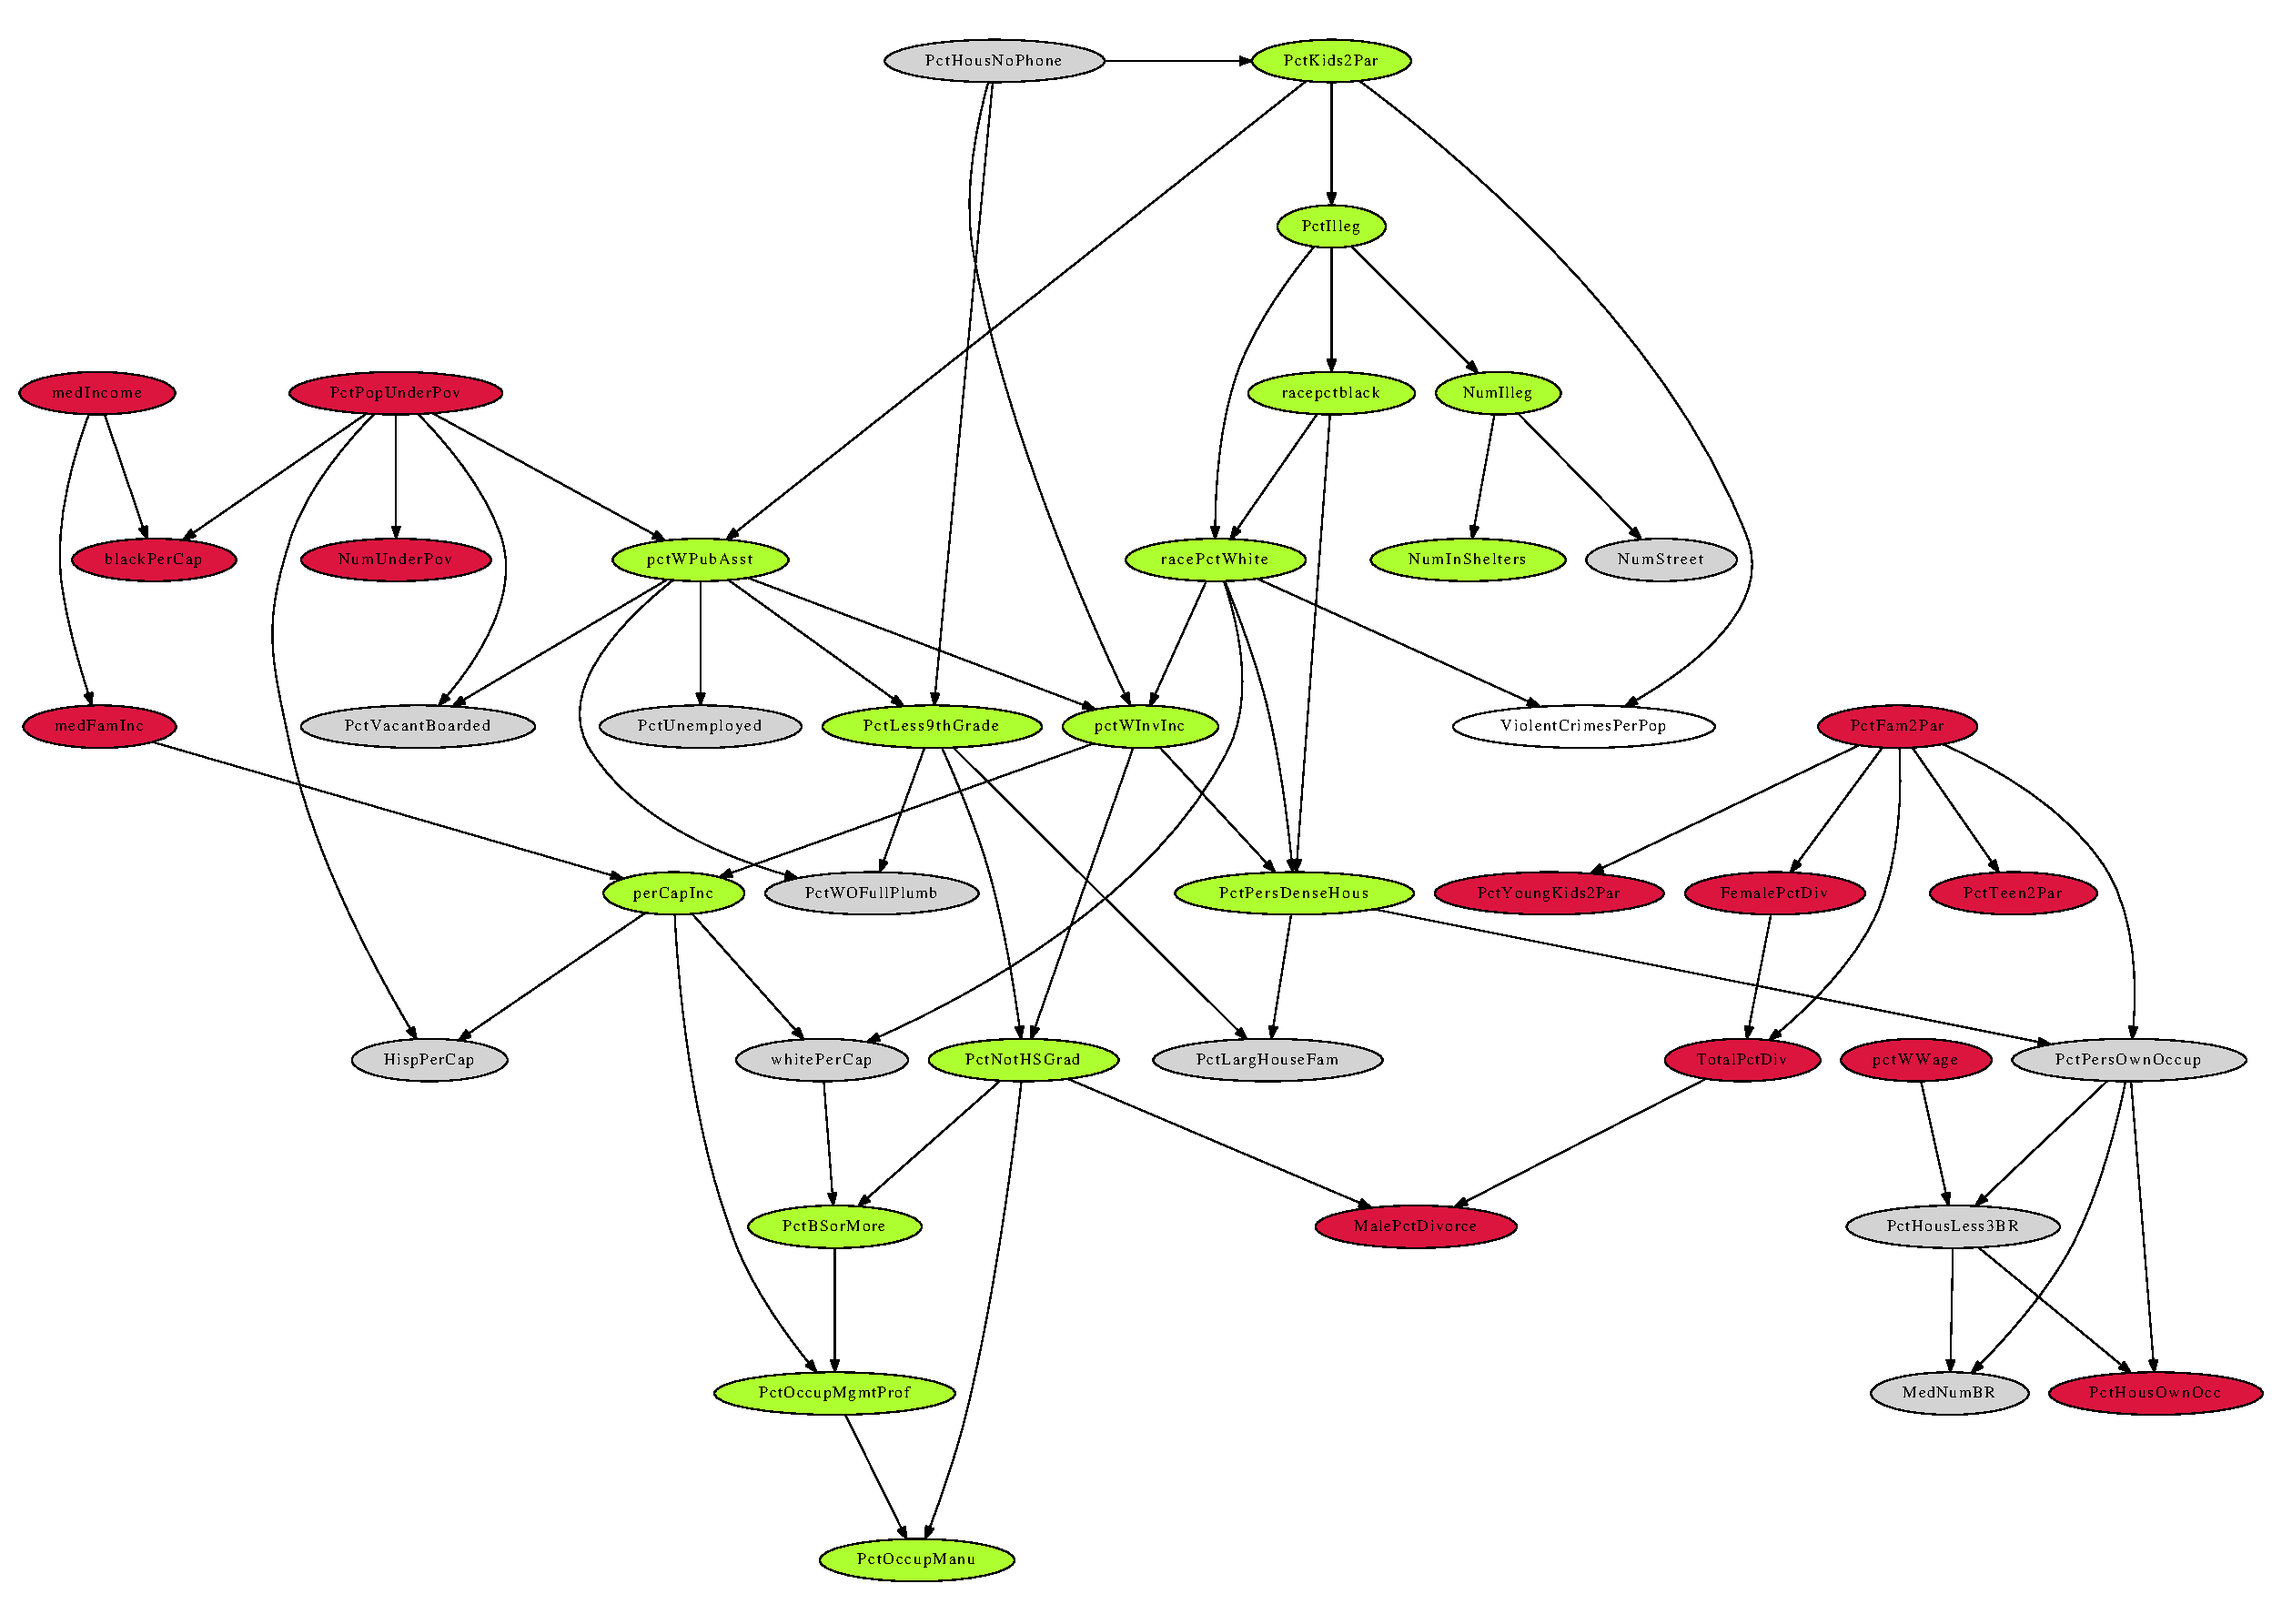
\includegraphics[scale=0.834]{fig/top-40_intersection_tolerance-1}
    \caption{Bayesian network for crime containing top 40 attributes with the highest crime impact factor.
    \\Legend: Green variables influence the $ViolentCrimesPerPop$ the same way as in the network with all 100 features. Influence of red variables is significantly different and therefore these variables shouldn't be considered.}
    \label{fig:crime_net_top40}
\end{figure}
\end{hugepage}

\begin{hugepage}
\pdfpagewidth=2\pdfpagewidth
\begin{figure}[h]
    \centering
    \vspace*{-2.5cm}
    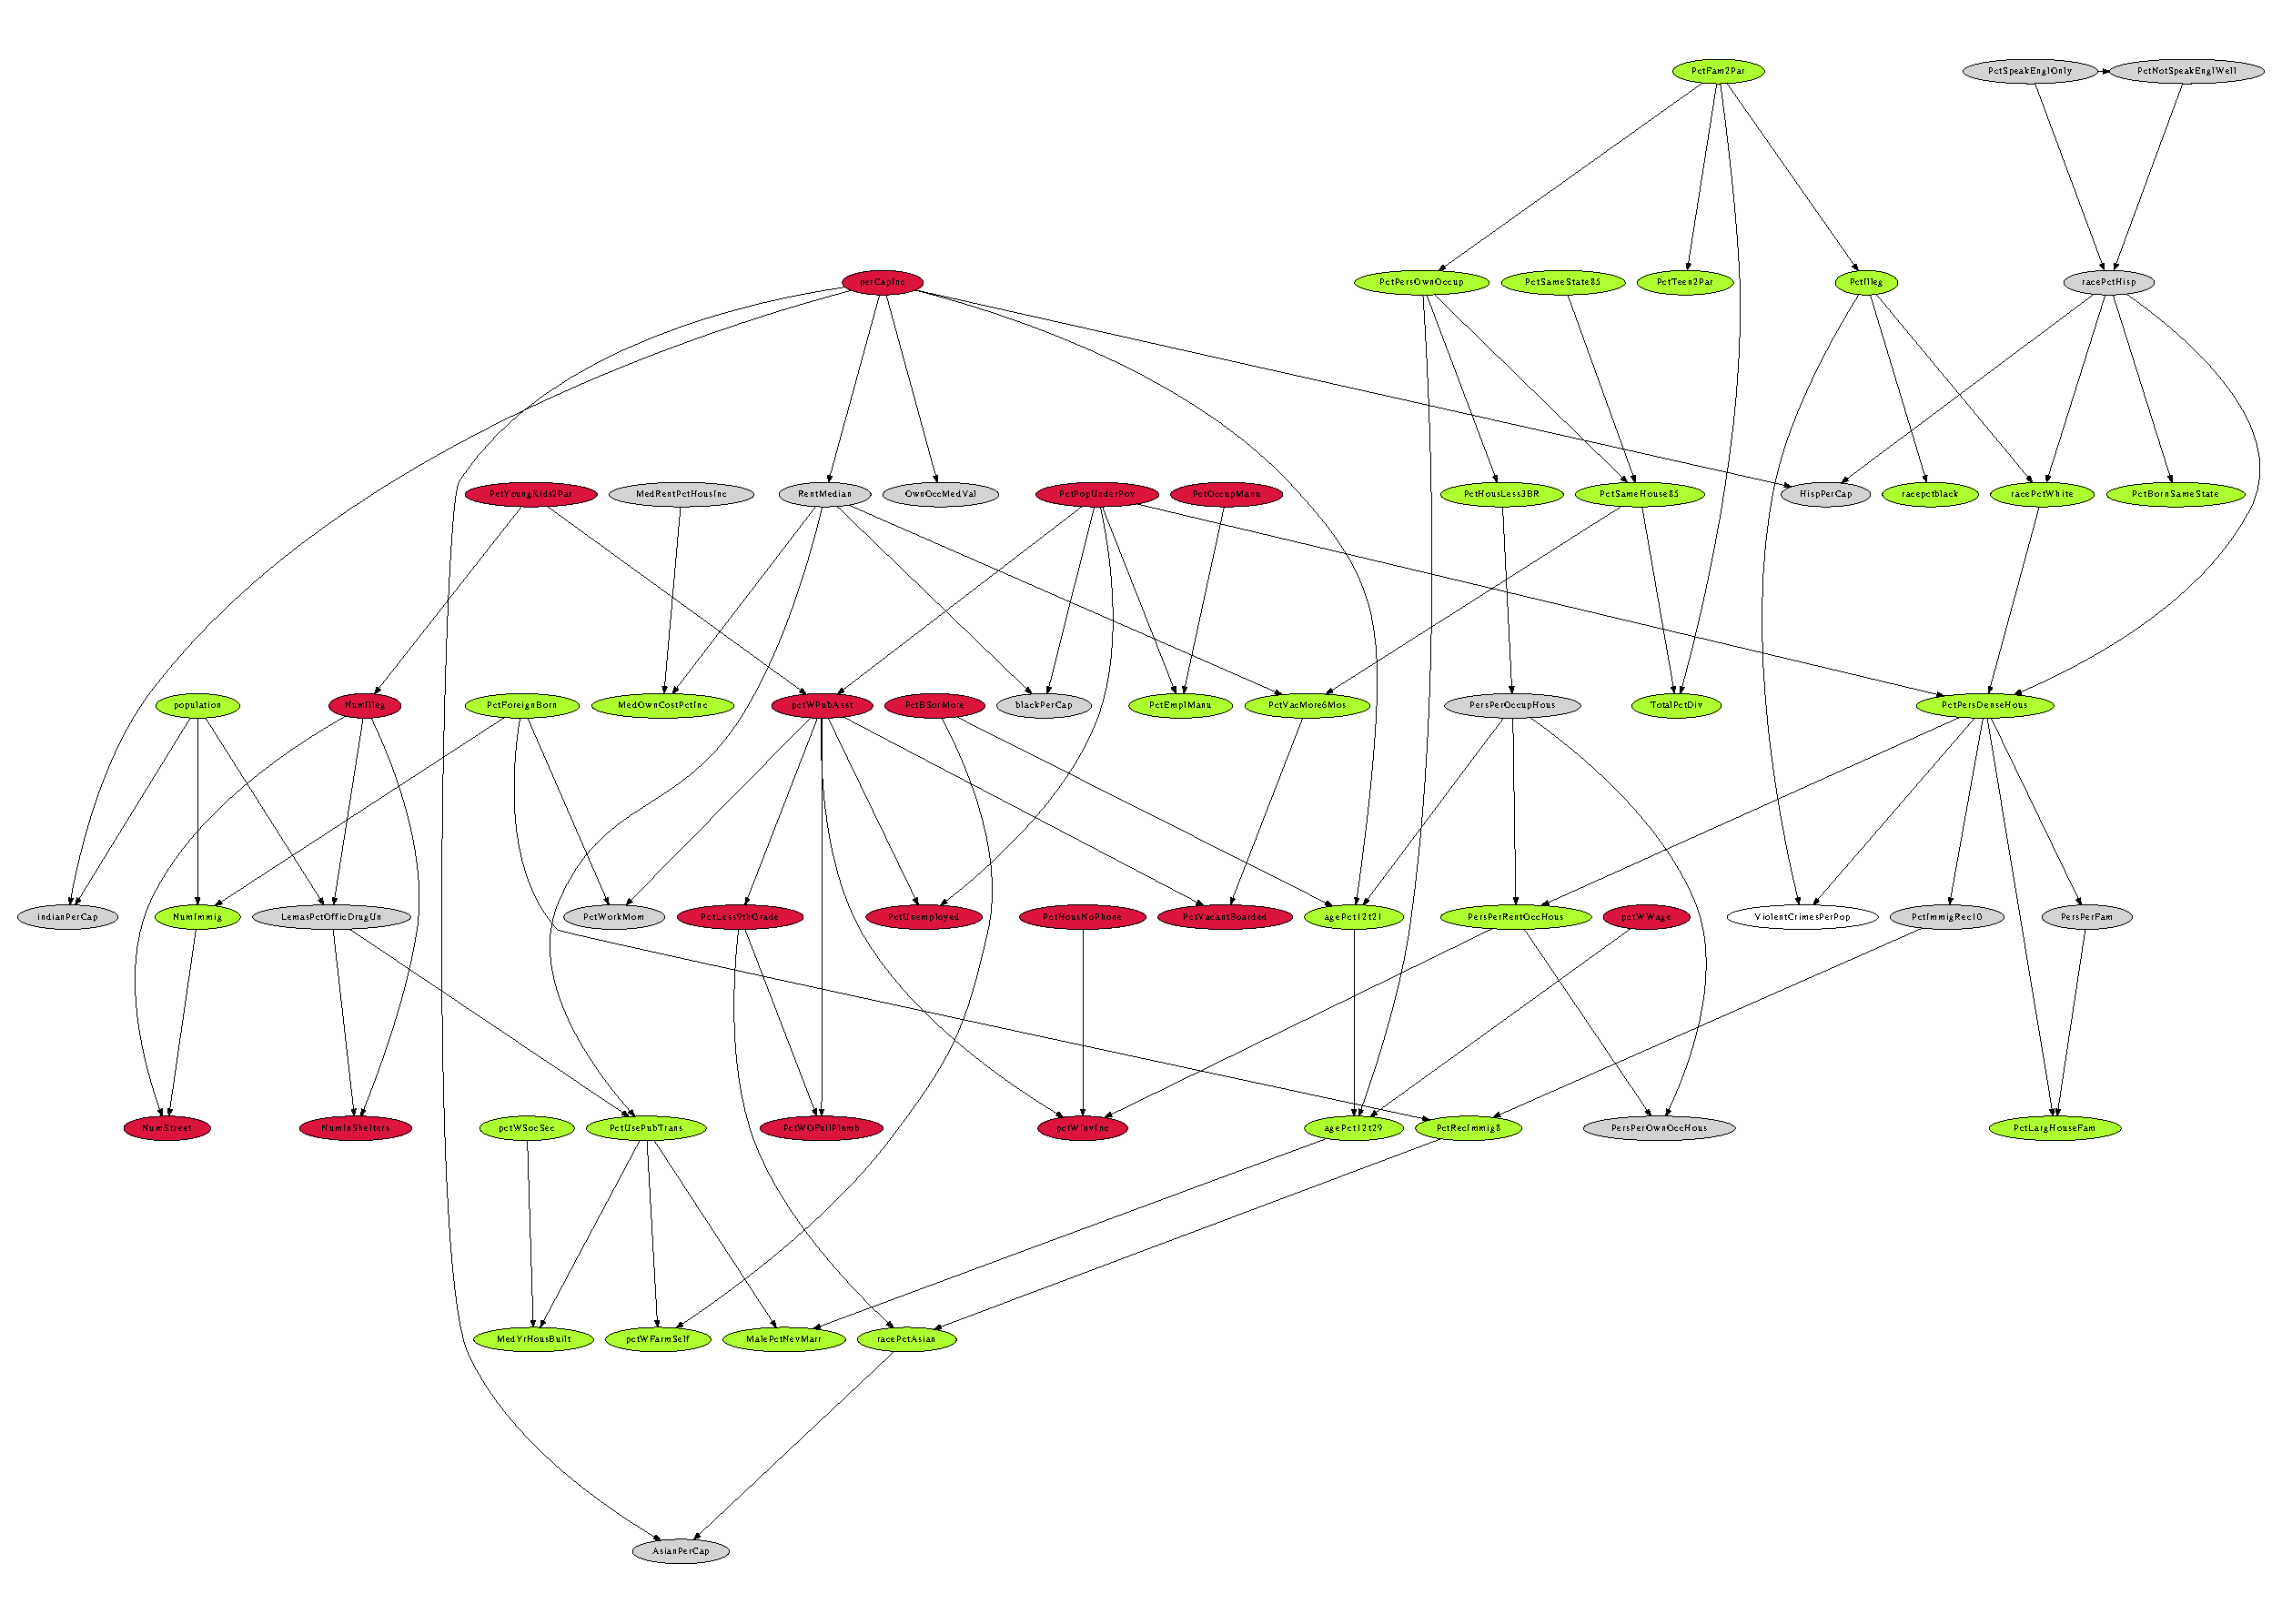
\includegraphics[scale=0.83]{fig/round-3_intersection_tolerance-1}
    \caption{Final Bayesian network for crime after three rounds of iterative elimination of similar variables.
    \\Legend: Green variables influence the $ViolentCrimesPerPop$ the same way as in the network with all 100 features. Influence of red variables is significantly different and therefore these variables shouldn't be considered.}
    \label{fig:crime_net_round3}
\end{figure}
\end{hugepage}

\begin{hugepage}
\pdfpagewidth=2\pdfpagewidth
\begin{figure}[h]
    \centering
    \vspace*{-2.5cm}
    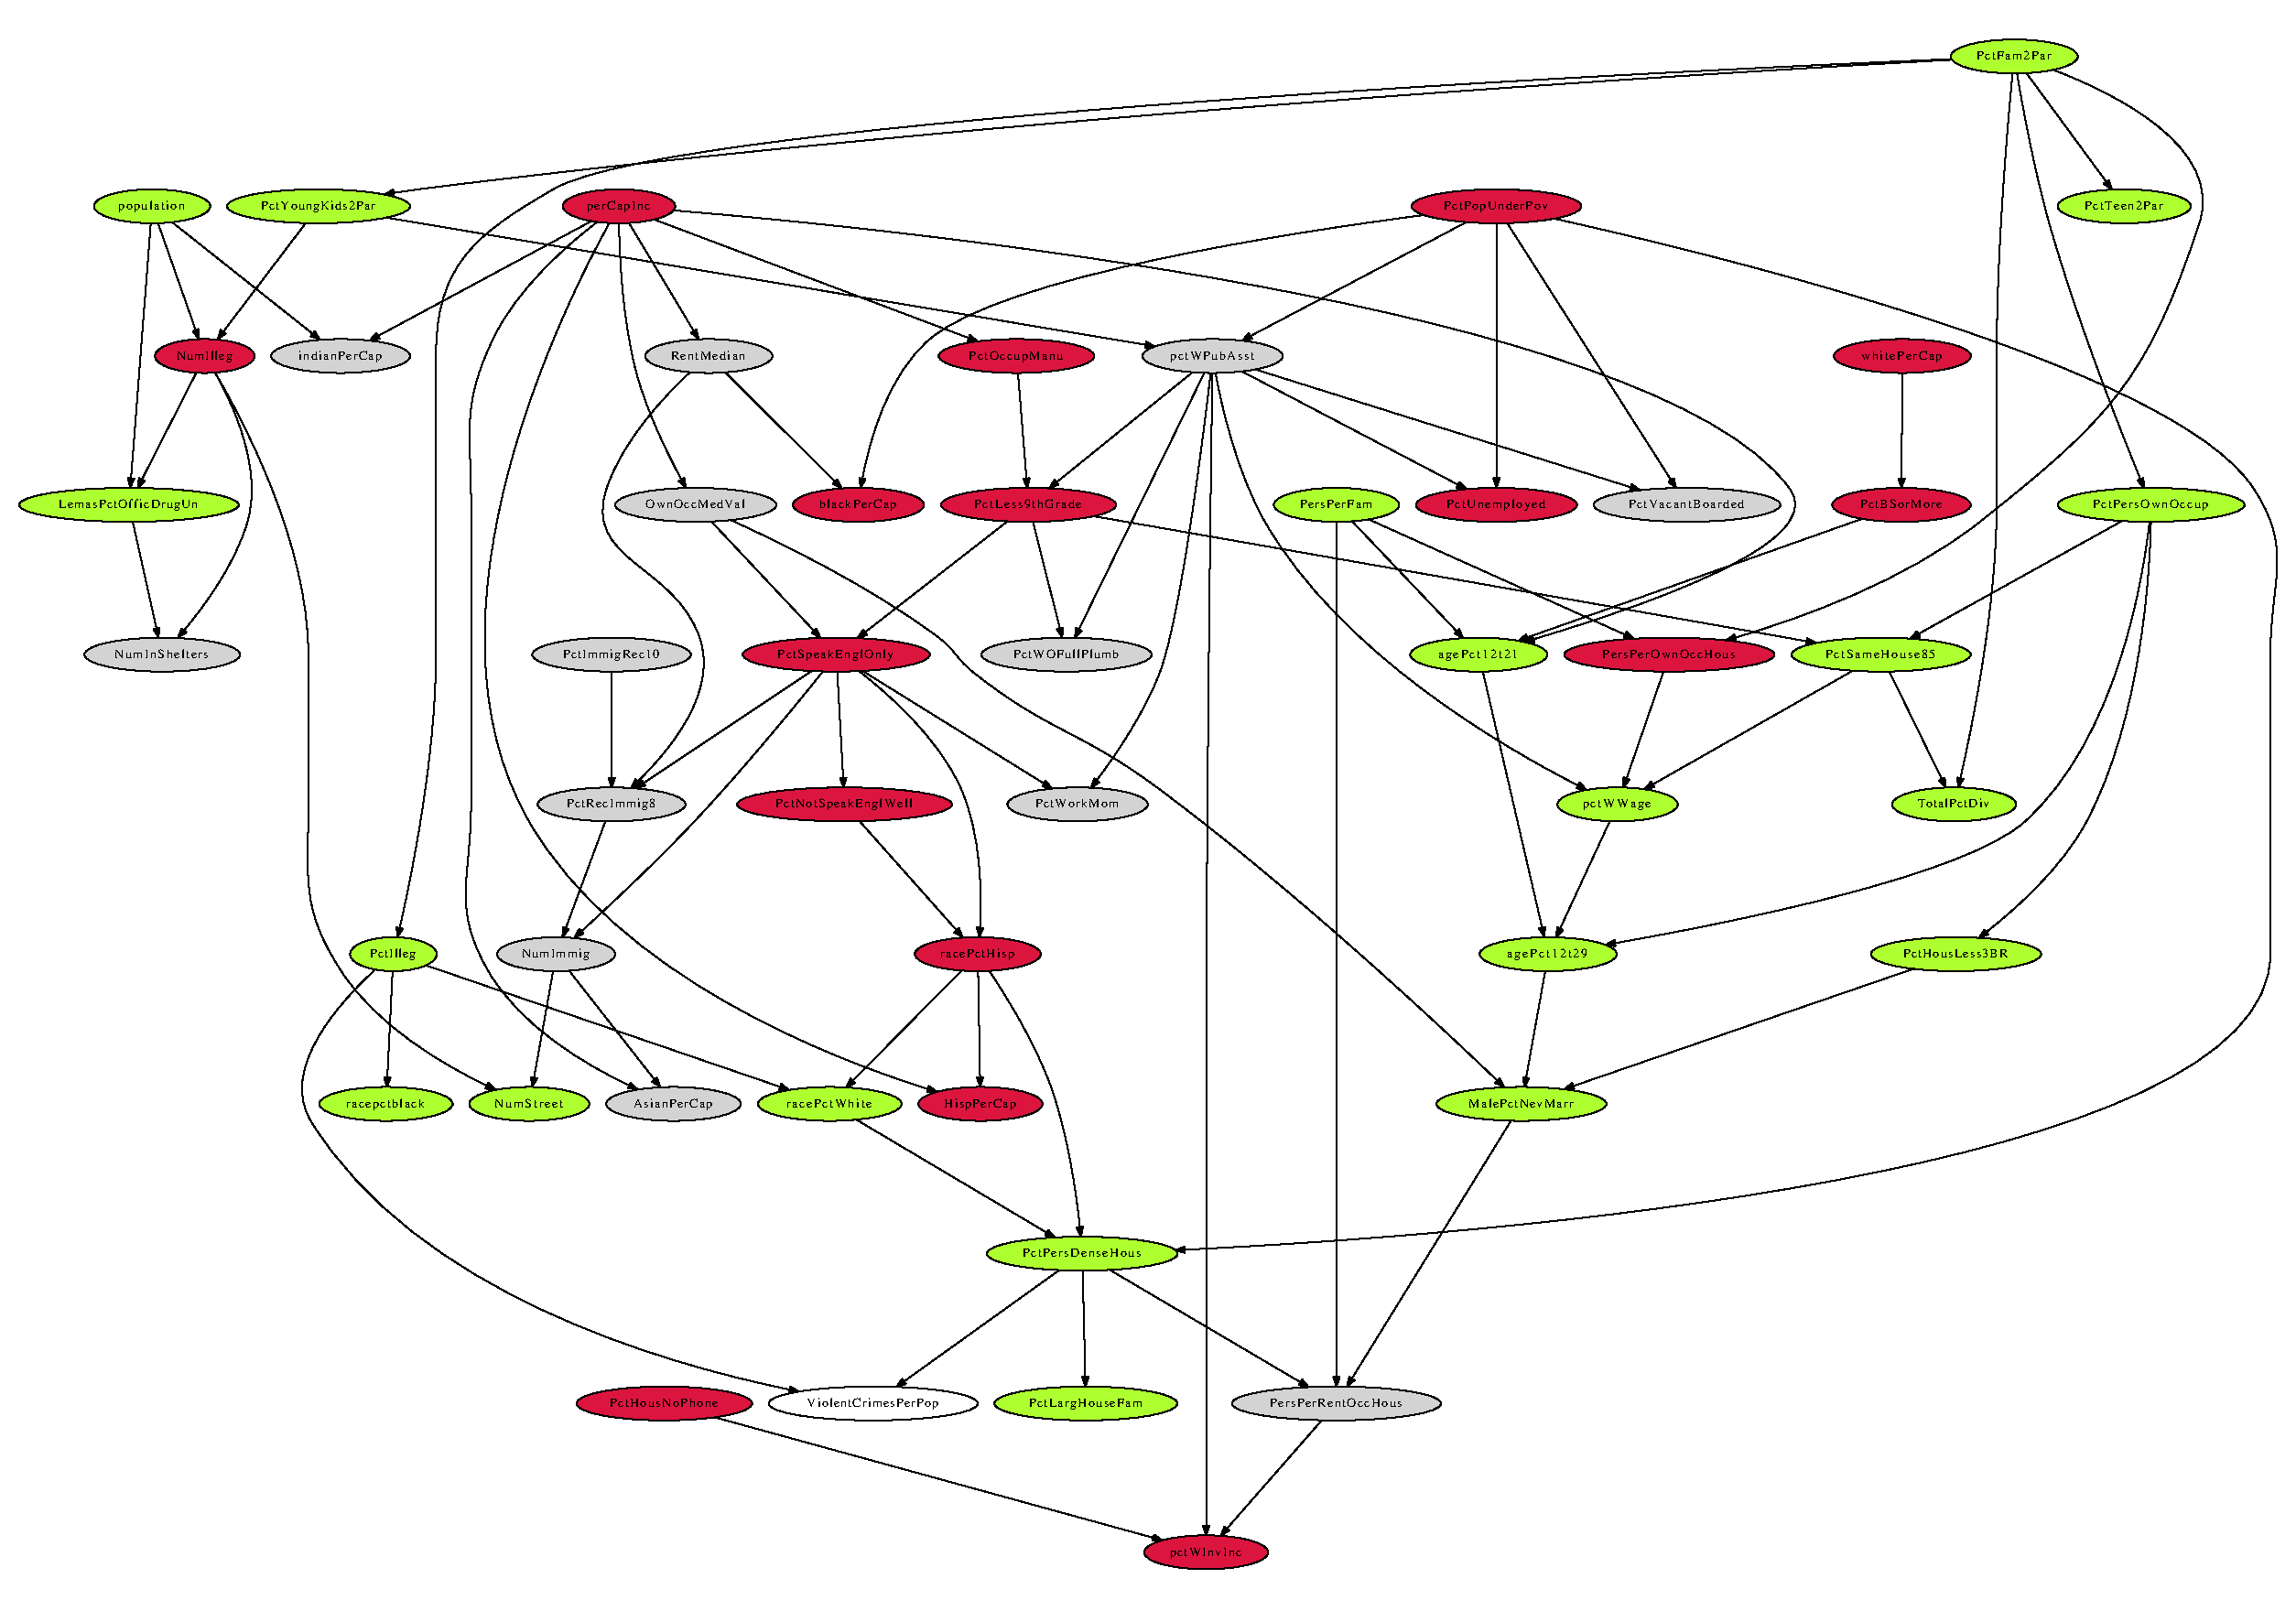
\includegraphics[scale=0.83]{fig/round-4_intersection_tolerance-1}
    \caption{Final Bayesian network for crime after three rounds of iterative elimination of similar variables and additional removal of variables whose crime impact factor is less than 0.07.
    \\Legend: Green variables influence the $ViolentCrimesPerPop$ the same way as in the network with all 100 features. Influence of red variables is significantly different and therefore these variables shouldn't be considered.}
    \label{fig:crime_net_round4}
\end{figure}
\end{hugepage}


 % viz. prilohy.tex
\end{document}
